% mnras_template.tex 
%
% LaTeX template for creating an MNRAS paper
%
% v3.0 released 14 May 2015
% (version numbers match those of mnras.cls)
%
% Copyright (C) Royal Astronomical Society 2015
% Authors:
% Keith T. Smith (Royal Astronomical Society)

% Change log
%
% v3.0 May 2015
%    Renamed to match the new package name
%    Version number matches mnras.cls
%    A few minor tweaks to wording
% v1.0 September 2013
%    Beta testing only - never publicly released
%    First version: a simple (ish) template for creating an MNRAS paper

%%%%%%%%%%%%%%%%%%%%%%%%%%%%%%%%%%%%%%%%%%%%%%%%%%
% Basic setup. Most papers should leave these options alone.
\documentclass[fleqn,usenatbib]{mnras}

% MNRAS is set in Times font. If you don't have this installed (most LaTeX
% installations will be fine) or prefer the old Computer Modern fonts, comment
% out the following line
\usepackage{newtxtext,newtxmath}
% Depending on your LaTeX fonts installation, you might get better results with one of these:
%\usepackage{mathptmx}
%\usepackage{txfonts}

% Use vector fonts, so it zooms properly in on-screen viewing software
% Don't change these lines unless you know what you are doing
\usepackage[T1]{fontenc}

% Allow "Thomas van Noord" and "Simon de Laguarde" and alike to be sorted by "N" and "L" etc. in the bibliography.
% Write the name in the bibliography as "\VAN{Noord}{Van}{van} Noord, Thomas"
\DeclareRobustCommand{\VAN}[3]{#2}
\let\VANthebibliography\thebibliography
\def\thebibliography{\DeclareRobustCommand{\VAN}[3]{##3}\VANthebibliography}


%%%%% AUTHORS - PLACE YOUR OWN PACKAGES HERE %%%%%

% Only include extra packages if you really need them. Common packages are:
\usepackage{graphicx}	% Including figure files
\usepackage{amsmath}	% Advanced maths commands
\usepackage{amssymb}	% Extra maths symbols

%%%%%%%%%%%%%%%%%%%%%%%%%%%%%%%%%%%%%%%%%%%%%%%%%%

%%%%% AUTHORS - PLACE YOUR OWN COMMANDS HERE %%%%%

% Please keep new commands to a minimum, and use \newcommand not \def to avoid
% overwriting existing commands. Example:
%\newcommand{\pcm}{\,cm$^{-2}$}	% per cm-squared

%%%%%%%%%%%%%%%%%%%%%%%%%%%%%%%%%%%%%%%%%%%%%%%%%%

%%%%%%%%%%%%%%%%%%% TITLE PAGE %%%%%%%%%%%%%%%%%%%

% Title of the paper, and the short title which is used in the headers.
% Keep the title short and informative.
\title[S-PLUS: H$\alpha$ fluxes for planetary nebulae]{S-PLUS: An atlas of integrated H$\alpha$ fluxes for planetary nebulae in the Magellanic Clouds}

% The list of authors, and the short list which is used in the headers.
% If you need two or more lines of authors, add an extra line using \newauthor
\author[L. G. Gutiérrez-Soto et al.]{
L. G. Gutiérrez-Soto,$^{1}$\thanks{E-mail: gsotoangel@fcaglp.unlp.edu.ar}
A. R. Lopes,$^{1}$
A. V. Smith Castelli$^{1,2}$
and S-PLUS people
\\
% List of institutions
$^{1}$Instituto de Astrof\'{i}sica de La Plata (CCT La Plata - CONICET - UNLP), B1900FWA, La Plata, Argentina\\
$^{2}$Facultad de Cs. Astronómicas y Geofísicas, UNLP, Paseo del Bosque S/N, B1900FWA, La Plata, Argentina
}

% These dates will be filled out by the publisher
\date{Accepted XXX. Received YYY; in original form ZZZ}

% Enter the current year, for the copyright statements etc.
\pubyear{2015}

% Don't change these lines
\begin{document}
\label{firstpage}
\pagerange{\pageref{firstpage}--\pageref{lastpage}}
\maketitle

% Abstract of the paper
\begin{abstract}
We present an atlas of integrated Halpha fluxes for planetary nebulae of the Magellanic Clouds (MC PNe) with measurements from the Southern Photometric Local Universe Survey (S-PLUS), a 12 band (7 narrow and 5 broad) imaging survey that allows us to perform an spatial analysis of the Halpha emission. Aperture photometry on the continuum-subtracted images was performed to extract Halpha + [N II] fluxes of the MC PNe observed by S-PLUS. The dust attenuation and [N II] contribution was corrected with empirical relations. Amongst its many applications, it can provide baseline data for photoionization and hydrodynamical modelling, and allow better estimates of Zanstra temperatures for PN central stars with accurate optical photometry. The weak nebular emission of the PNe were also analyzed to investigate the structure of the MC PNe further, for which the Halpha surface brightness was estimated. The densities in the nebulae of the PNe were also measured using the previously estimated surface brightness. These results were compared with previous measurements from the literature. The preliminary results of this study are present in this contribution.
\end{abstract}

% Select between one and six entries from the list of approved keywords.
% Don't make up new ones.
\begin{keywords}
planetary nebulae: general -- ISM: lines and bands -- surveys
\end{keywords}

%%%%%%%%%%%%%%%%%%%%%%%%%%%%%%%%%%%%%%%%%%%%%%%%%%

%%%%%%%%%%%%%%%%% BODY OF PAPER %%%%%%%%%%%%%%%%%%

\section{Introduction}

The Small Magellanic Cloud (SMC) is a gas-rich late-type dwarf galaxy \citep{Bolatto:2007}
with a gas-to-dust ratio 30 times higher than the Milky Way (Stanimirovic et al. 2000).
The SMC is one of the closest and most prominent neighbors of the Milky Way, is a southern hemisphere dwarf galaxy of low mass ($M_\text{dyn} \sim 2.4\times 10^{9}$M$\odot$; \citealp{Stanimirovi:2004}) and and small size ($R_{*} \sim 3$ kpc).
It is a member of the Local Group and is classified as an irregular galaxy (ImIV$-$V)
(Sandage et al. 1994). The SMC is at a distance of 60.6$\pm$3.8 kpc (Hilditch et al. 2005)
from the Galaxy which makes the spatial scale $\sim$0.3 pc$/$arcsec.


\section{Methodology}
\label{sec:metho}
\subsection{Observations: the S-PLUS project}
\label{sec:obser}

\begin{figure*}
    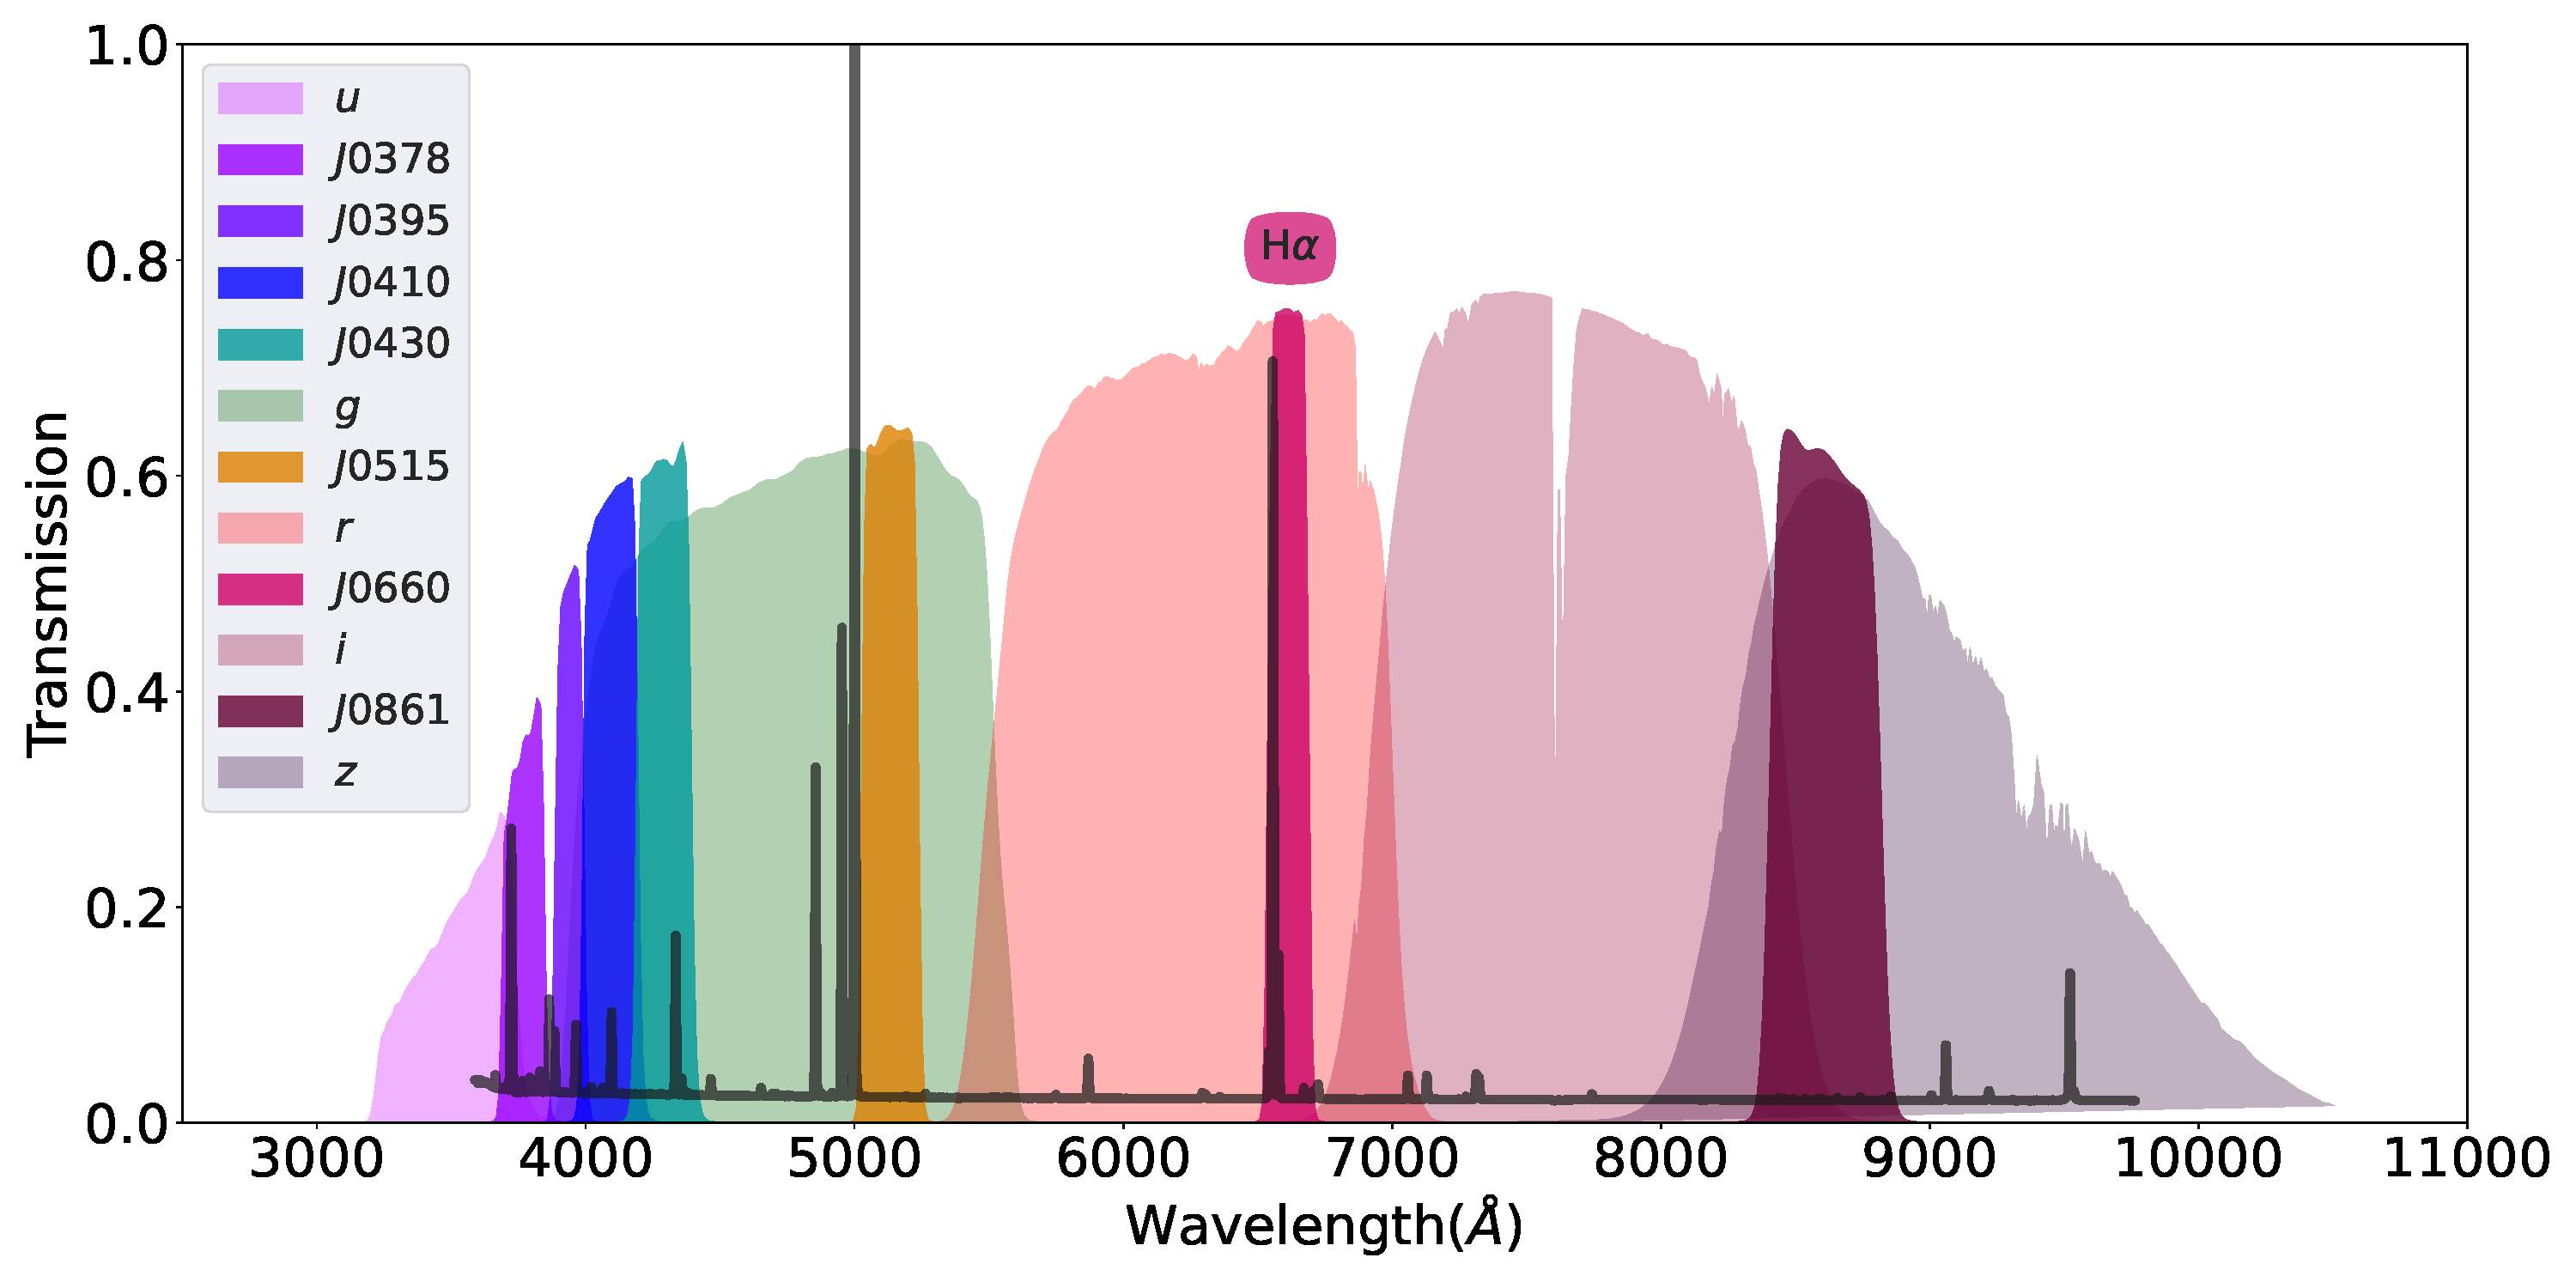
\includegraphics[width=0.8\linewidth]{Figs/splus-filter-pn}
    \caption{Transmission curves of the S-PLUS filter set. The narrow-band filter
      $J0660$ includes the H$\alpha$ emission line. Over-plotted is a spectra of typical SMC PN.}
    \label{fig:curves}
\end{figure*}

This manuscript uses data from the S-PLUS DR4, which covers 3,000 square degrees of the southern sky. The S-PLUS DR4 can be accessed in the database of the project, \texttt{S-PLUS Cloud}\footnote{\url{https://splus.cloud/}}. S-PLUS is being carried out by a dedicated 0.83m robotic telescope located at Cerro Tololo, Chile \citep{Mendes:2019}.
The project is surveying the southern sky using the 12 filters from the so-called Javalambre filter system \citep{Marin-Franch:2012}, which spans the wavelength range from 3000\AA\ to 10000\AA. The system includes seven narrow-band filters
(\textit{J}0378, \textit{J}0395, \textit{J}0410, \textit{J}0430,
\textit{J}0515, \textit{J}0660,  and \textit{J}0861) 
and five broad-band Sloan-like \citep{Fukugita:1996} filters (see Fig. \ref{fig:curves}).
%(\(u, g, r, i~\mathrm{and}~z\)).
The narrow-band $J0660$ filter used in S-PLUS is centred at lambda 6614~\AA~and has a width of about 147~\AA~(Table 2 of \citealp{Mendes:2019}), and therefore it  covers both 
the H{$\alpha$} and the doublet [N II] \(\lambda\lambda 6548,6584\)  spectral lines for sources up to a redshift of approximately 0.02.

\subsection{PNe in the Magellanic Clouds}

\begin{figure*}
    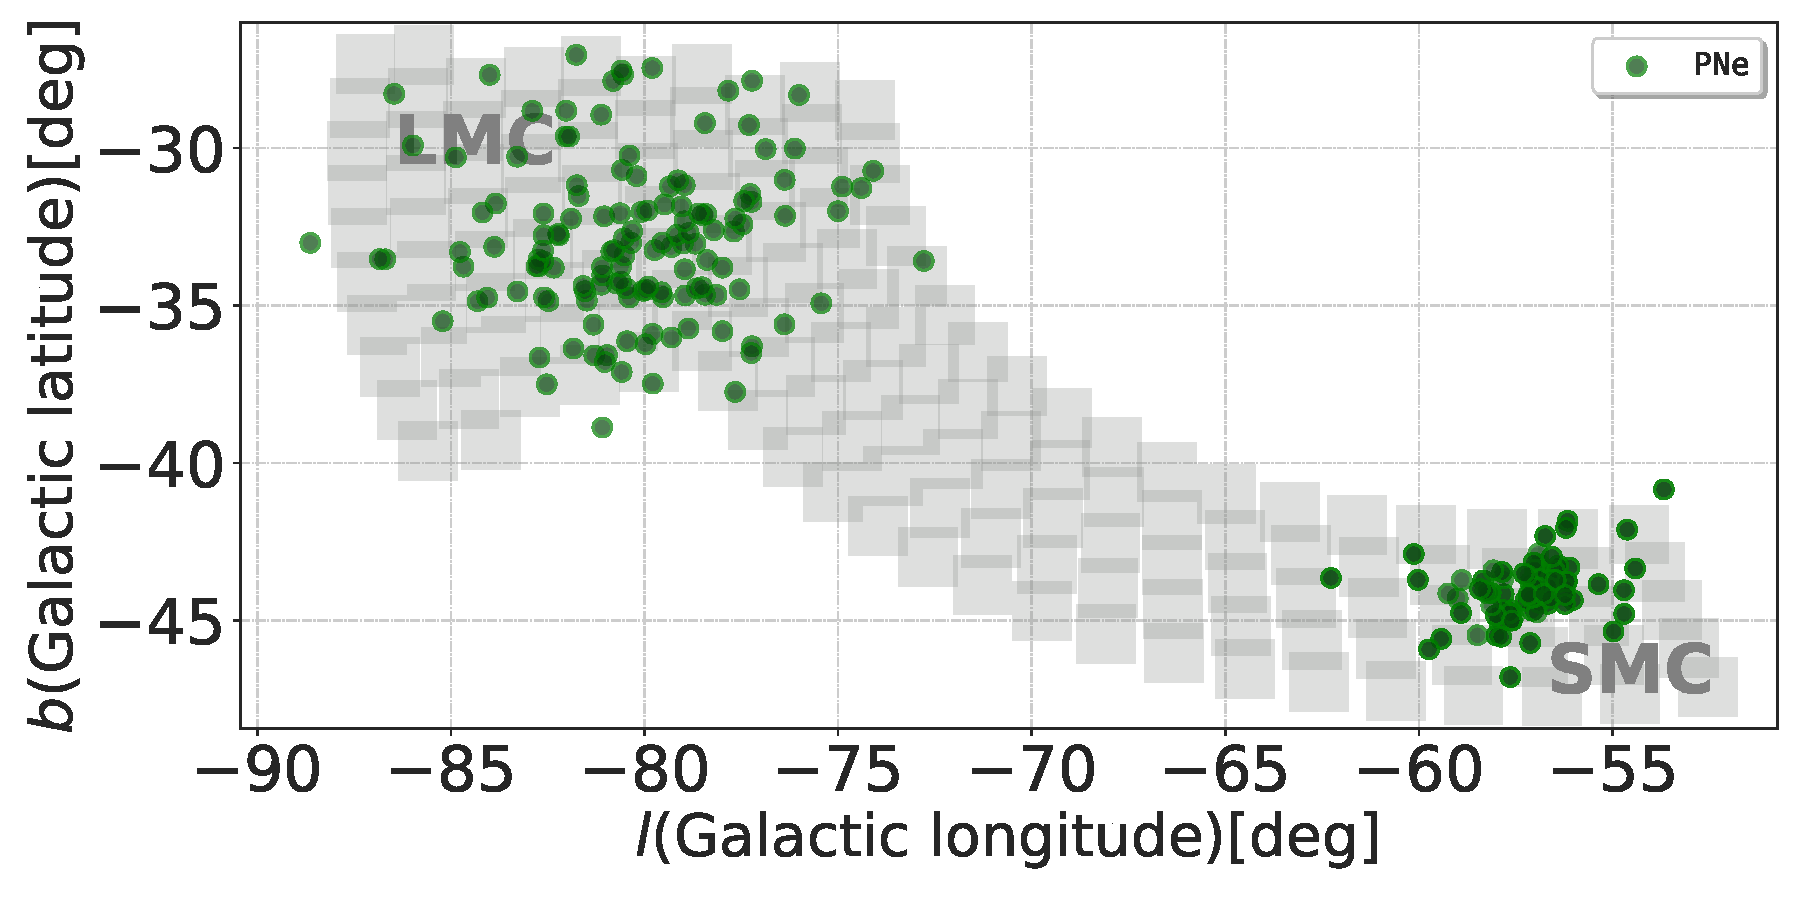
\includegraphics[width=\linewidth]{Figs/galactic-coord-pn.pdf}
    \caption{Transmission curves of the S-PLUS filter set. The narrow-band filter
      $J0660$ includes the H$\alpha$ emission line. Over-plotted is a spectra of typical SMC PN.}
    \label{fig:pn_mc}
\end{figure*}


\section{Results}


\section{Conclusions}



\section*{Acknowledgements}

The Acknowledgements section is not numbered. Here you can thank helpful
colleagues, acknowledge funding agencies, telescopes and facilities used etc.
Try to keep it short.

%%%%%%%%%%%%%%%%%%%%%%%%%%%%%%%%%%%%%%%%%%%%%%%%%%
\section*{Data Availability}

 
The inclusion of a Data Availability Statement is a requirement for articles published in MNRAS. Data Availability Statements provide a standardised format for readers to understand the availability of data underlying the research results described in the article. The statement may refer to original data generated in the course of the study or to third-party data analysed in the article. The statement should describe and provide means of access, where possible, by linking to the data or providing the required accession numbers for the relevant databases or DOIs.




%%%%%%%%%%%%%%%%%%%% REFERENCES %%%%%%%%%%%%%%%%%%

% The best way to enter references is to use BibTeX:

\bibliographystyle{mnras}
\bibliography{ref} % if your bibtex file is called example.bib


% Alternatively you could enter them by hand, like this:
% This method is tedious and prone to error if you have lots of references
%\begin{thebibliography}{99}
%\bibitem[\protect\citeauthoryear{Author}{2012}]{Author2012}
%Author A.~N., 2013, Journal of Improbable Astronomy, 1, 1
%\bibitem[\protect\citeauthoryear{Others}{2013}]{Others2013}
%Others S., 2012, Journal of Interesting Stuff, 17, 198
%\end{thebibliography}

%%%%%%%%%%%%%%%%%%%%%%%%%%%%%%%%%%%%%%%%%%%%%%%%%%

%%%%%%%%%%%%%%%%% APPENDICES %%%%%%%%%%%%%%%%%%%%%

\appendix

\section{Some extra material}

If you want to present additional material which would interrupt the flow of the main paper,
it can be placed in an Appendix which appears after the list of references.

%%%%%%%%%%%%%%%%%%%%%%%%%%%%%%%%%%%%%%%%%%%%%%%%%%


% Don't change these lines
\bsp	% typesetting comment
\label{lastpage}
\end{document}

% End of mnras_template.tex
